\chapter{Modélisation UML}
\section{Philosophie de modélisation}
La modélisation UML sert à rendre la cible fonctionnelle vérifiable. Les diagrammes ne doivent pas seulement illustrer le rapport ; ils doivent permettre de contrôler que chaque besoin métier possède un acteur, un processus, des interactions et, lorsque nécessaire, un composant applicatif.

\begin{figure}[H]
\centering
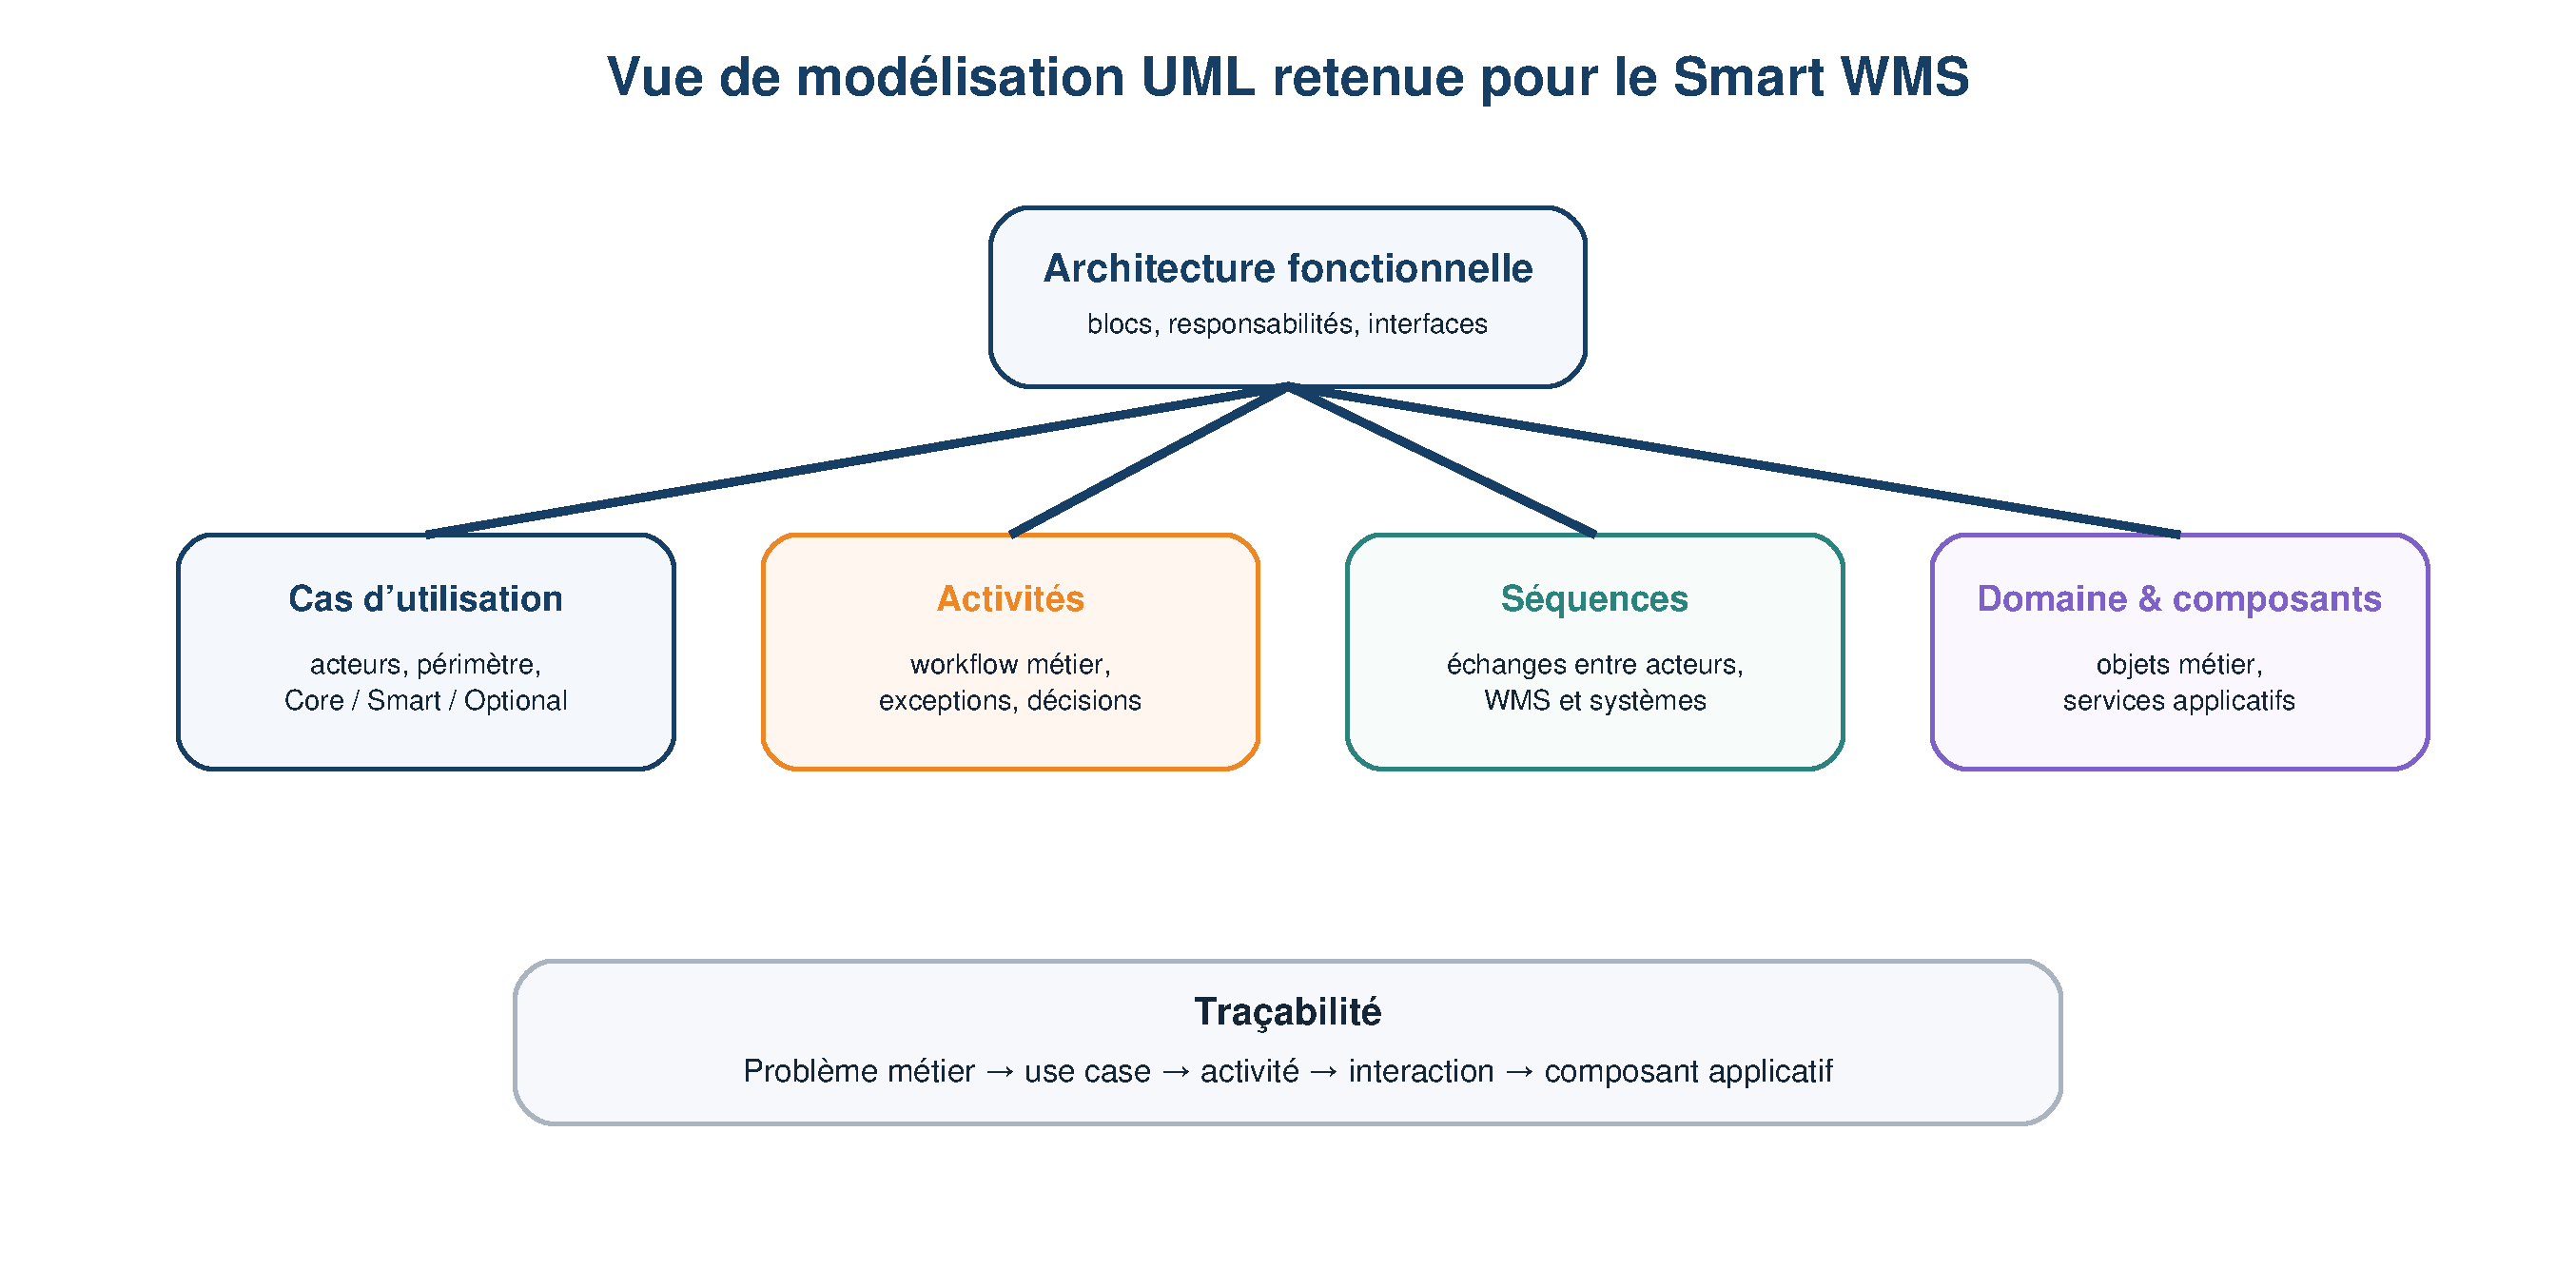
\includegraphics[width=0.92\linewidth]{figures/chapitre5/vue_modelisation_uml.pdf}
\caption{Vue de modélisation UML retenue pour le Smart WMS.}
\label{fig:vue-uml}
\end{figure}

\section{Diagrammes de cas d'utilisation}
Les diagrammes de cas d'utilisation sont organisés par domaine : vue globale, réception, stockage et inventaire, préparation et expédition, services transversaux, yard et ressources. La correction principale consiste à séparer visuellement les use cases Core, Smart et Optional. Les blocs Données de référence et Stockage des données ne sont pas représentés comme des cas d'utilisation déclenchés par un acteur ; ils relèvent du modèle de domaine et du diagramme de composants.

\section{Diagrammes d'activité}
Les diagrammes d'activité décrivent les flux de bout en bout : réception intelligente, stockage et inventaire, expédition, supervision énergétique et environnementale. Leur intérêt est de montrer les alternatives : règle métier standard lorsqu'aucune infrastructure avancée n'est disponible, puis activation OCR, caméra 3D, RFID, WCS/WES ou BMS/EMS lorsque le contexte le permet.

\section{Modèle de domaine et composants}
Le modèle de domaine doit couvrir les objets nécessaires à la cohérence métier : Warehouse, Zone, Location, Product, ProductRequirement, StockUnit, HandlingUnit, Lot, CustomerOrder, OrderLine, Task, Worker, Equipment, Device, Sensor, SensorReading, Alert et Recommendation. Le diagramme de composants traduira ensuite ces objets en services : services métier WMS, services Smart, intégrations externes, couche données et couche terrain.

Les sources PlantUML utilisées pour cette modélisation sont conservées en annexe afin de faciliter les itérations futures.
